%-----------------------------------------------------------------------------------------------------------%
\newpage

\setcounter{chapter}{2}
\setcounter{example}{0}
\setcounter{eqtn}{0}
\setcounter{section}{0}


\chapter{\lr{\textbf{جبر ماتریسی}}}
\textbf{\vspace{-140pt}}
\begin{figure}[H]
    \centering
    \setlength{\belowcaptionskip}{-10pt}
    
\includegraphics[width=0.8\textwidth]{Images/4/2/4.Session.1.2.0}
    \label{fig:4.Session.1.2.0}
\end{figure}
\textbf{\vspace{20pt}}
{
    \Large
    \begin{spacing}{1.5}
        در گرافیک کامپیوتری سه‌بعدی، ما از ماتریس‌ها برای توصیف فشرده تبدیل‌های هندسی مانند تغییر مقیاس، دوران و انتقال و همچنین برای تغییر مختصات یک نقطه یا بردار از یک سیستم مختصات به سیستم مختصات دیگر استفاده می‌کنیم.
        این فصل به بررسی ریاضیات ماتریس‌ها می‌پردازد.
        \\

        \textbf{\LARGE \hspace{-40pt}اهداف:}
        \begin{enumerate}[label=\textbf{\arabic*}.]
            \item {به دست آوردن درک درستی از ماتریس‌ها و عملیات تعریف شده بر روی آن‌ها.}
            \item {یادگیری اینکه چگونه ضرب بردار-ماتریس را می‌توان به عنوان یک ترکیب خطی مشاهده کرد.}
            \item {یادگیری اینکه ماتریس همانی چیست و ترانهاده، دترمینان و معکوس یک ماتریس چیست.}
            \item {برای آشنایی با زیرمجموعه کلاس‌ها و توابع ارائه شده توسط کتابخانه ریاضی \lr{DirectX} که برای ریاضیات ماتریسی استفاده می‌شود.}
        \end{enumerate}
    \end{spacing}
}
%-----------------------------------------------------------------------------------------------------------%
\newpage

\setcounter{figure}{0}
\renewcommand{\thefigure}{\arabic{figure}.\arabic{chapter}}


\section{\textbf{تعریف}}
\label{sec:2.1}
{
    \Large
    \begin{spacing}{1.5}
        $\textbf{M}$ ماتریس $m\times n$، یک آرایه مستطیلی از اعداد حقیقی با $m$ ردیف و $n$ ستون است.
        حاصل ضرب تعداد سطرها و ستون ها، ابعاد ماتریس را نشان می‌دهد.
        اعداد موجود در یک ماتریس را عنصر، ورودی یا درایه می‌نامند.
        ما یک عنصر ماتریسی را با مشخص کردن سطر و ستون عنصر با استفاده از نماد دوگانه $\textbf{M}_{ij}$ شناسایی می‌کنیم،
        جایی که زیرنویس اول ردیف و زیرنویس دوم ستون را مشخص می‌کند.

        \begin{example}{exp:2.1}
            \Large
            ماتریس‌های زیر را در نظر بگیرید:\\\\
            $\textbf{A}=\begin{bmatrix}
                            3.5 & 0  & 0                      & 0 \\
                            0   & 1  & 0                      & 0 \\
                            0   & 0  & 0.5                    & 0 \\
                            2   & -5 & \sqrt{\displaystyle 2} & 1
            \end{bmatrix}, \textbf{B}=\begin{bmatrix}
                                          B_{11} & B_{12} \\
                                          B_{21} & B_{22} \\
                                          B_{31} & B_{32}
            \end{bmatrix}, \textbf{u}=[u_{1},u_{2},u_{3}], \textbf{v}=\begin{bmatrix}
                                                                          1                      \\
                                                                          2                      \\
                                                                          \sqrt{\displaystyle 3} \\
                                                                          \pi
            \end{bmatrix}$
            \\
            \begin{enumerate}[label=\textbf{\arabic*}.]
                \item {ماتریس $\textbf{A}$ یک ماتریس $4\times 4$ است؛
                ماتریس $\textbf{B}$ یک ماتریس $3\times 2$ است؛
                ماتریس $\textbf{u}$ یک ماتریس $1\times 3$ است؛
                و ماتریس $\textbf{v}$ یک ماتریس $4\times 1$ است.}
                \item {عنصر ردیف چهارم و ستون دوم ماتریس $\textbf{A}$ را با $A_{42}=-5$ شناسایی می‌کنیم. عنصر ردیف دوم و ستون اول ماتریس $\textbf{B}$ را با $B_{21}$ شناسایی می‌کنیم.}
                \item {ماتریس‌های $\textbf{u}$ و $\textbf{v}$ ماتریس‌های خاصی هستند به این معنا که به ترتیب حاوی یک سطر یا ستون هستند.
                ما گاهی اوقات این نوع ماتریس‌ها را بردار ردیف یا بردار ستون می‌نامیم زیرا برای نمایش یک بردار به شکل ماتریس استفاده می‌شوند
                    (به عنوان مثال، می‌توانیم آزادانه نمادهای برداری $(x, y, z)$ و $[x, y, z]$ را مبادله کنیم).
                    توجه داشته باشید که برای بردارهای ردیف و ستون، استفاده از یک زیرنویس دوگانه برای نشان دادن عناصر ماتریس غیر‌ضروری است (ما فقط به یک زیرنویس نیاز داریم.)}
            \end{enumerate}
            گاهی اوقات ما ردیف‌های یک ماتریس را به عنوان بردار در نظر میگیریم. برای مثال، ممکن است بنویسیم:

            \begin{center}
                $\begin{bmatrix}
                     A_{11} & A_{12} & A_{13} \\
                     A_{21} & A_{22} & A_{23} \\
                     A_{31} & A_{32} & A_{33}
                \end{bmatrix}=\begin{bmatrix}
                                  \leftarrow & A_{1,*} & \rightarrow \\
                                  \leftarrow & A_{2,*} & \rightarrow \\
                                  \leftarrow & A_{3,*} & \rightarrow
                \end{bmatrix}$
            \end{center}

            که $\textbf{A}_{1,*}=[A_{11},A_{12},A_{13}]$، $\textbf{A}_{2,*}=[A_{21},A_{22},A_{23}]$ و $\textbf{A}_{3,*}=[A_{31},A_{32},A_{33}]$ هستند.
            در این نماد، اندیس اول سطر را مشخص می‌کند و در اندیس دوم یک ’*‘ قرار می‌دهیم تا نشان دهد ما به کل بردار سطر اشاره می‌کنیم. به همین ترتیب، ما همین کار را برای ستون‌ها انجام دهیم:

            \begin{center}
                $\begin{bmatrix}
                     A_{11} & A_{12} & A_{13} \\
                     A_{21} & A_{22} & A_{23} \\
                     A_{31} & A_{32} & A_{33}
                \end{bmatrix}=\begin{bmatrix}
                                  \uparrow   & \uparrow   & \uparrow   \\
                                  A_{*,1}    & A_{*,2}    & A_{*,3}    \\
                                  \downarrow & \downarrow & \downarrow
                \end{bmatrix}$
            \end{center}

            که

            \begin{center}
                $\textbf{A}_{*,1}=\begin{bmatrix}
                                      A_{11} \\
                                      A_{21} \\
                                      A_{31}
                \end{bmatrix},
                \textbf{A}_{*,2}=\begin{bmatrix}
                                     A_{12} \\
                                     A_{22} \\
                                     A_{32}
                \end{bmatrix},
                \textbf{A}_{*,3}=\begin{bmatrix}
                                     A_{13} \\
                                     A_{23} \\
                                     A_{33}
                \end{bmatrix}$
            \end{center}

            در این نماد، اندیس دوم ستون را مشخص می‌کند و در اولین نمایه یک ’*‘ قرار می‌دهیم تا نشان دهد ما به کل بردار ستون اشاره می‌کنیم.

            \textbf{اکنون برابری، جمع، ضرب اسکالر و تفریق را بر روی ماتریس‌ها تعریف می‌کنیم:}

            \begin{enumerate}[label=\textbf{\arabic*}.]
                \item {دو ماتریس برابر هستند اگر و تنها اگر عناصر متناظر آن‌ها برابر باشند.
                به این ترتیب، دو ماتریس باید تعداد سطر و ستون یکسانی داشته باشند تا با هم مقایسه شوند.}
                \item {ما دو ماتریس را با اضافه کردن عناصر متناظر آن‌ها جمع می‌کنیم.
                به این ترتیب، جمع ماتریس‌هایی با تعداد سطر و ستون یکسان تنها منطقی است.}
                \item {ما یک اسکالر و یک ماتریس را با ضرب اسکالر در هر عنصر ماتریس ضرب می‌کنیم.}
                \item {ما تفریق را بر حسب جمع ماتریس و ضرب اسکالر تعریف می‌کنیم. یعنی \\ $\textbf{A}-\textbf{B}=\textbf{A}+(-1\cdot\textbf{B})=\textbf{A}+(-\textbf{B})$.}
            \end{enumerate}
        \end{example}

        \begin{example}{exp:2.2}
            \Large
            فرض کنید
            \begin{center}
                $\textbf{A}=\begin{bmatrix}
                                1  & 5 \\
                                -2 & 3
                \end{bmatrix}, \textbf{B}=\begin{bmatrix}
                                              6 & 2  \\
                                              5 & -8
                \end{bmatrix}, \textbf{C}=\begin{bmatrix}
                                              1  & 5 \\
                                              -2 & 3
                \end{bmatrix}, \textbf{D}=\begin{bmatrix}
                                              2  & 1 & -3 \\
                                              -6 & 3 & 0
                \end{bmatrix}$
            \end{center}
            \textbf{\vspace{12pt}}
            پس،
            \lr{
                \begin{enumerate}[label=(\roman*) ]
                    \item {
                        $\textbf{A}+\textbf{B}=\begin{bmatrix}
                                                   1  & 5 \\
                                                   -2 & 3
                        \end{bmatrix}+\begin{bmatrix}
                                          6 & 2  \\
                                          5 & -8
                        \end{bmatrix}=\begin{bmatrix}
                                          1+6  & 5+2    \\
                                          -2+5 & 3+(-8)
                        \end{bmatrix}=\begin{bmatrix}
                                          7 & 7  \\
                                          3 & -5
                        \end{bmatrix}$
                    } \textbf{\vspace{6pt}}
                    \item {
                        $\textbf{A}=\textbf{C}$
                    } \textbf{\vspace{12pt}}
                    \item {
                        $3\textbf{D}=3\begin{bmatrix}
                                          2  & 1 & -3 \\
                                          -6 & 3 & 0
                        \end{bmatrix}=\begin{bmatrix}
                                          3(2)  & 3(1) & 3(-3) \\
                                          3(-6) & 3(3) & 3(0)
                        \end{bmatrix}=\begin{bmatrix}
                                          6   & 3 & -9 \\
                                          -18 & 9 & 0
                        \end{bmatrix}$
                    } \textbf{\vspace{12pt}}
                    \item {
                        $\textbf{A}-\textbf{B}=\begin{bmatrix}
                                                   1  & 5 \\
                                                   -2 & 3
                        \end{bmatrix}-\begin{bmatrix}
                                          6 & 2  \\
                                          5 & -8
                        \end{bmatrix}=\begin{bmatrix}
                                          1-6  & 5-2    \\
                                          -2-5 & 3-(-8)
                        \end{bmatrix}=\begin{bmatrix}
                                          -5 & 3  \\
                                          -7 & 11
                        \end{bmatrix}$
                    }
                \end{enumerate}
            }

            از آنجایی که جمع و ضرب اسکالر به صورت عنصری انجام می‌شود، ماتریس‌ها اساساً ویژگی‌های جمع و ضرب اسکالر زیر را از اعداد حقیقی به ارث می‌برند:

            \lr{
                \begin{enumerate}[label=(\roman*) ]
                    \item {$\textbf{A}+\textbf{B}=\textbf{B}+\textbf{A}$\hspace{35 mm} \rl{\textbf{(}خاصیت جابجایی جمع\textbf{)}}}
                    \item {$(\textbf{A}+\textbf{B})+\textbf{C}=\textbf{A}+(\textbf{B}+\textbf{C})$\hspace{6 mm} \rl{\textbf{(}خاصیت شرکت پذیری جمع\textbf{)}}}
                    \item {$r(\textbf{A}+\textbf{B})=r\textbf{A}+r\textbf{B}$\hspace{26 mm} \rl{\textbf{(}خاصیت تویع پذیری اسکالر روی ماتریس\textbf{)}}}
                    \item {$(r+s)\textbf{A}=r\textbf{A}+s\textbf{A}$\hspace{26 mm} \rl{\textbf{(}خاصیت تویع پذیری ماتریس روی اسکالر\textbf{)}}}
                \end{enumerate}
            }
        \end{example}
    \end{spacing}
}


\section{\textbf{ضرب ماتریس}}
\label{sec:2.2}
\subsection{\textbf{تعریف}}
\label{subsec:2.2.1}
{
    \Large
    \begin{spacing}{1.5}
        اگر $\textbf{A}$ یک ماتریس $m\times n$ و $\textbf{B}$ یک ماتریس $n\times p$ باشد،
        حاصلضرب $\textbf{AB}$ که یک ماتریس $m\times p$ است، با $\textbf{C}$ تعریف می‌شود،
        که در آن ورودی $ij$ ام از $\textbf{C}$ حاصل، با گرفتن ضرب داخلی بردار ردیف $i$ ام $\textbf{A}$ با بردار ستون $j$ ام $\textbf{B}$ به دست می‌آید، یعنی

        \begin{eqtn}{eqtn:2.1}
            \centering
            $\textbf{C}_{ij}=\textbf{A}_{i,*}\cdot\textbf{B}_{*,j}$
        \end{eqtn}

        بنابراین توجه داشته باشید برای اینکه حاصلضرب ماتریس $\textbf{AB}$ تعریف شود، ما نیاز داریم که تعداد ستون‌های $\textbf{A}$ برابر با تعداد ردیف‌های $\textbf{B}$ باشد،
        به این معنا که باید بُعد بردارهای ردیف در $\textbf{A}$ با بُعد بردارهای ستون در $\textbf{B}$ برابر باشد.
        اگر این ابعاد مطابقت نداشتند، آنگاه ضرب داخلی در معادله \ref{eqtn:2.1} معنی نخواهد داشت.

        \begin{example}{exp:2.3}
            \Large
            فرض کنید

            \begin{center}
                $\textbf{A}=\begin{bmatrix}
                                1  & 5 \\
                                -2 & 3
                \end{bmatrix}, \textbf{B}=\begin{bmatrix}
                                              2  & -6 \\
                                              1  & 3  \\
                                              -3 & 0
                \end{bmatrix}$
            \end{center}

            حاصلضرب $\textbf{AB}$ تعریف نشده است زیرا بردارهای ردیف در $\textbf{A}$ دارای بُعد $2$ و بردارهای ستون در $\textbf{B}$ دارای بُعد $3$ هستند.
            همچنین نمیتوان بردار ردیف اول $\textbf{A}$ را با بردار ستون اول $\textbf{B}$  ضرب داخلی کرد زیرا نمیتوان ضرب داخلی بردار دو‌بعدی با بردار سه‌بعدی را گرفت.
        \end{example}

        \begin{example}{exp:2.4}
            \Large
            فرض کنید

            \begin{center}
                $\textbf{A}=\begin{bmatrix}
                                -1 & 5 & -4 \\
                                3  & 2 & 1
                \end{bmatrix}, \textbf{B}=\begin{bmatrix}
                                              2  & 1  & 0 \\
                                              0  & -2 & 1 \\
                                              -1 & 2  & 3
                \end{bmatrix}$
            \end{center}

            ابتدا اشاره می‌کنیم که حاصلضرب $\textbf{AB}$ تعریف شده است (و یک ماتریس $2\times 3$ است) زیرا تعداد ستون‌های $\textbf{A}$ با تعداد ردیف‌های $\textbf{B}$ برابر است. با معادله \ref{eqtn:2.1} نتیجه می‌گیریم:
            \begin{equation*}
                \centering
                \begin{split}
                    \textbf{AB}&=\begin{bmatrix}
                                     -1 & 5 & -4 \\
                                     3  & 2 & 1
                    \end{bmatrix}\begin{bmatrix}
                                     2  & 1  & 0 \\
                                     0  & -2 & 1 \\
                                     -1 & 2  & 3
                    \end{bmatrix}\\
                    &={\large\begin{bmatrix}
                    (-1,5,-4)
                                 \cdot(2,1,0)         & (-1,5,-4)\cdot(1,-2,2) & (-1,5,-4)\cdot(0,1,3) \\
                                 (3,2,1)\cdot(2,0,-1) & (3,2,1)\cdot(1,-2,2)   & (3,2,1)\cdot(0,1,3)
                    \end{bmatrix}}\\
                    &=\begin{bmatrix}
                          2 & -19 & -7 \\
                          5 & 1   & 5
                    \end{bmatrix}
                \end{split}
            \end{equation*}

            توجه کنید که حاصلضرب $\textbf{BA}$ تعریف نشده است زیرا تعداد ستون‌های $\textbf{B}$ با تعداد ردیف‌های $\textbf{A}$ برابر نیست. یعنی $\textbf{AB}\neq\textbf{BA}$.
        \end{example}

    \end{spacing}
}

\subsection{\textbf{ضرب بردار-ماتریس}}
\label{subsec:2.2.2}
{
    \Large
    \begin{spacing}{1.5}
        ضرب ماتریس بردار زیر را در نظر بگیرید:

        \begin{center}
            $\textbf{uA}=[x,y,z]\begin{bmatrix}
                                    A_{11} & A_{12} & A_{13} \\
                                    A_{21} & A_{22} & A_{23} \\
                                    A_{31} & A_{32} & A_{33}
            \end{bmatrix}=[x,y,z]\begin{bmatrix}
                                     \uparrow   & \uparrow   & \uparrow   \\
                                     A_{*,1}    & A_{*,2}    & A_{*,3}    \\
                                     \downarrow & \downarrow & \downarrow
            \end{bmatrix}$
        \end{center}

        توجه داشته باشید که $\textbf{uA}$ در این مورد به یک بردار ردیف $1\times 3$ ارزیابی می‌شود.
        اکنون با اعمال معادله \ref{eqtn:2.1} به دست می‌آید:
        \begin{equation*}
            \centering
            \begin{split}
                \textbf{uA}&=\begin{bmatrix}
                                 \textbf{u}\cdot\textbf{A}_{*,1} & \textbf{u}\cdot\textbf{A}_{*,2} & \textbf{u}\cdot\textbf{A}_{*,3}
                \end{bmatrix}\\
                &=[xA_{11}+yA_{21}+zA_{31},\hspace{3 mm} xA_{12}+yA_{22}+zA_{32},\hspace{3 mm} xA_{13}+yA_{23}+zA_{33}] \\
                &=[xA_{11},xA_{12},xA_{13}]+[yA_{21},yA_{22},yA_{23}]+[zA_{31},zA_{32},zA_{33}] \\
                &=x[A_{11},A_{12},A_{13}]+y[A_{21},A_{22},A_{23}]+z[A_{31},A_{32},A_{33}] \\
                &=x\textbf{A}_{1,*}+y\textbf{A}_{2,*}+z\textbf{A}_{3,*}
            \end{split}
        \end{equation*}
        پس،

        \begin{eqtn}{eqtn:2.2}
            \centering
            $\textbf{uA}=x\textbf{A}_{1,*}+y\textbf{A}_{2,*}+z\textbf{A}_{3,*}$
        \end{eqtn}

        معادله \ref{eqtn:2.2} نمونه‌ای از ترکیب خطی است و
        می‌گوید که حاصلضرب ماتریس برداری $\textbf{uA}$ معادل یک ترکیب خطی از بردارهای ردیف ماتریس $\textbf{A}$ با ضرایب اسکالر $x$، $y$ و $z$ است که توسط بردار $\textbf{u}$ داده شده است.
        توجه داشته باشید که، اگرچه ما این را برای یک بردار ردیف $1\times 3$ و یک ماتریس $3\times 3$ نشان دادیم، نتیجه به طور کلی درست است.
        یعنی برای یک $1\times n$ بردار ردیف $\textbf{u}$ و یک ماتریس $n\times m$ $\textbf{A}$، داریم که $\textbf{uA}$ ترکیبی خطی از بردارهای ردیف در $\textbf{A}$ با ضرایب اسکالر داده شده توسط $\textbf{u}$ است:

        \begin{eqtn}{eqtn:2.3}
            \centering
            $[u_{1},\dots,u_{n}]\begin{bmatrix}
                                    A_{11} & \cdots & A_{13} \\
                                    \vdots & \ddots & \vdots \\
                                    A_{31} & \cdots & A_{33}
            \end{bmatrix}=u_{1}\textbf{A}_{1,*}+\dots+u_{n}\textbf{A}_{n,*}$
        \end{eqtn}
    \end{spacing}
}

\subsection{\textbf{شرکت پذیری}}
\label{subsec:2.2.3}
{
    \Large
    \begin{spacing}{1.5}
        ضرب ماتریس دارای ویژگی‌های جبری خوبی است. برای مثال، ضرب ماتریسی بر جمع توزیع پذیر است: $\textbf{A}(\textbf{B}+\textbf{C})=\textbf{AB}+\textbf{AC}$ و $(\textbf{A}+\textbf{B})\textbf{C}=\textbf{AC}+\textbf{BC}$.
        به طور خاص، ما از قانون شرکت پذیری ضرب ماتریس گاه به گاه استفاده خواهیم کرد، که به ما امکان می‌دهد ترتیب ضرب ماتریس‌ها را انتخاب کنیم:

        \begin{center}
            $(\textbf{AB})\textbf{C}=\textbf{A}(\textbf{BC})$
        \end{center}

    \end{spacing}
}


\section{\textbf{ترانهاده‌ی یک ماتریس}}
\label{sec:2.3}
{
    \Large
    \begin{spacing}{1.5}
        ترانهاده یک ماتریس با تعویض ردیف‌ها و ستون‌های ماتریس پیدا می‌شود.
        بنابراین ترانهاده یک ماتریس $m\times n$ یک ماتریس $n\times m$ است.
        جابجایی یک ماتریس $\textbf{M}$ را $\textbf{M}^T$ نشان می‌دهیم.

        \begin{example}{exp:2.5}
            \Large
            ترانهاده سه ماتریس زیر را بیابید:\\

            \begin{center}
                $\textbf{A}=\begin{bmatrix}
                                2 & -1 & 8  \\
                                3 & 6  & -4
                \end{bmatrix}, \textbf{B}=\begin{bmatrix}
                                              a & b & c \\
                                              d & e & f \\
                                              g & h & i
                \end{bmatrix}, \textbf{C}=\begin{bmatrix}
                                              1 \\
                                              2 \\
                                              3 \\
                                              4
                \end{bmatrix}$
            \end{center}

            برای تکرار، ترانهاده‌ها با تعویض ردیف‌ها و ستون‌ها پیدا می‌شوند، بنابراین

            \begin{center}
                $\textbf{A}^T=\begin{bmatrix}
                                  2  & 3  \\
                                  -1 & 6  \\
                                  8  & -4
                \end{bmatrix}, \textbf{B}^T=\begin{bmatrix}
                                                a & d & g \\
                                                b & e & h \\
                                                c & f & i
                \end{bmatrix}, \textbf{C}^T=\begin{bmatrix}
                                                1 & 2 & 3 & 4
                \end{bmatrix}$
            \end{center}

            ترانهاده دارای خواص مفید زیر است:
            \lr{
                \begin{enumerate}[label=(\roman*) ]
                    \item {$(\textbf{A}+\textbf{B})^T=\textbf{A}^T+\textbf{B}^T$}
                    \item {$(c\textbf{A})^T=c\textbf{A}^T$}
                    \item {$(\textbf{A}\textbf{B})^T=\textbf{B}^T\textbf{A}^T$}
                    \item {$(\textbf{A}^T)^T=\textbf{A}$}
                    \item {$(\textbf{A}^{-1})^T=(\textbf{A}^T)^{-1}$}
                \end{enumerate}
            } \textbf{\vspace{-30pt}}
        \end{example}
    \end{spacing}
}


\section{\textbf{ماتریس همانی}}
\label{sec:2.4}
{
    \Large
    \begin{spacing}{1.5}
        ماتریس خاصی به نام ماتریس همانی وجود دارد.
        ماتریس همانی یک ماتریس مربعی است که همه عناصر به جز در قطر اصلی صفر و عناصر قطر اصلی همه یک هستند.
        به عنوان مثال،
%        در زیر ماتریس‌های همانی $2\times 2$، $3\times 3$ و $4\times 4$ آمده است:
        \begin{center}
            $\begin{bmatrix}
                 1 & 0 \\
                 0 & 1
            \end{bmatrix}, \begin{bmatrix}
                               1 & 0 & 0 \\
                               0 & 1 & 0 \\
                               0 & 0 & 1
            \end{bmatrix}, \begin{bmatrix}
                               1 & 0 & 0 & 0 \\
                               0 & 1 & 0 & 0 \\
                               0 & 0 & 1 & 0 \\
                               0 & 0 & 0 & 1
            \end{bmatrix}$
        \end{center}

        ماتریس همانی به عنوان $1$ در ضرب عمل می‌کند.
        یعنی اگر $\textbf{A}$ یک ماتریس $m\times n$ باشد، $\textbf{B}$ یک ماتریس $n\times p$ باشد و $\textbf{I}$ ماتریس همانی $n\times n$ باشد، پس

        \begin{center}
            $\textbf{AI}=\textbf{A}, \textbf{IB}=\textbf{B}$
        \end{center}

        به عبارت دیگر، ضرب یک ماتریس در ماتریس همانی، ماتریس را تغییر نمی‌دهد.
        ماتریس همانی را می‌توان به عنوان عدد $1$ برای ماتریس‌ها در نظر گرفت.
        به ویژه، اگر $\textbf{M}$ یک ماتریس مربعی باشد، ضرب با ماتریس همانی جابجایی پذیر است:

        \begin{center}
            $\textbf{MI}=\textbf{IM}=\textbf{M}$
        \end{center}

        \begin{example}{exp:2.6}
            \Large
            فرض کنید
            $\textbf{M}=\begin{bmatrix}
                            1 & 2 \\
                            0 & 4
            \end{bmatrix}, \textbf{I}=\begin{bmatrix}
                                          1 & 0 \\
                                          0 & 1
            \end{bmatrix}$
            باشد، درستی $\textbf{MI}=\textbf{IM}=\textbf{M}$ را چک کنید.

            اعمال \ref{eqtn:2.1} نتیجه میدهد:

            \begin{center}
                $\textbf{MI}=\begin{bmatrix}
                                 1 & 2 \\
                                 0 & 4
                \end{bmatrix}\begin{bmatrix}
                                 1 & 0 \\
                                 0 & 1
                \end{bmatrix}=\begin{bmatrix}
                (1,2)
                                  \cdot(1,0)      & (1,2)\cdot(0,1) \\
                                  (0,4)\cdot(1,0) & (0,4)\cdot(0,1)
                \end{bmatrix}=\begin{bmatrix}
                                  1 & 2 \\
                                  0 & 4
                \end{bmatrix},$
            \end{center}
            \begin{center}
                $\textbf{IM}=\begin{bmatrix}
                                 1 & 0 \\
                                 0 & 1
                \end{bmatrix}\begin{bmatrix}
                                 1 & 2 \\
                                 0 & 4
                \end{bmatrix}=\begin{bmatrix}
                (1,0)
                                  \cdot(1,0)      & (1,0)\cdot(2,4) \\
                                  (1,0)\cdot(1,0) & (0,1)\cdot(2,4)
                \end{bmatrix}=\begin{bmatrix}
                                  1 & 2 \\
                                  0 & 4
                \end{bmatrix}$
            \end{center}

            بنابراین $\textbf{MI}=\textbf{IM}=\textbf{M}$ درست است.
        \end{example}

        \begin{example}{exp:2.7}
            \Large
            فرض کنید
            $\textbf{u}=[-1,2], \textbf{I}=\begin{bmatrix}
                                               1 & 0 \\
                                               0 & 1
            \end{bmatrix}$
            درستی $\textbf{uI}=\textbf{u}$ را چک کنید.

            اعمال \ref{eqtn:2.1} نتیجه میدهد:

            $\textbf{uI}=[-1,2]\begin{bmatrix}
                                   1 & 0 \\
                                   0 & 1
            \end{bmatrix}=\left[ (-1,2)\cdot(1,0), (-1,2)\cdot(1,0) \right]=[-1, 2]$

            توجه داشته باشید که ما نمی‌توانیم حاصل ضرب \textbf{Iu} را بگیریم زیرا ضرب ماتریس تعریف نشده است.
        \end{example}
    \end{spacing}
}


\section{\textbf{دترمینان یک ماتریس}}
\label{sec:2.5}
{
    \Large
    \begin{spacing}{1.3}
        دترمینان تابع خاصی است که یک ماتریس مربعی را دریافت و یک عدد حقیقی را خروجی می‌دهد.
        دترمینان یک ماتریس مربعی $\textbf{A}$ معمولاً با \lr{det $\textbf{A}$} نشان داده می‌شود.
        می‌توان نشان داد که دترمینان دارای تفسیر هندسی مربوط به حجم جعبه‌ها است و اطلاعاتی در مورد چگونگی تغییر حجم‌ها تحت تبدیل‌های خطی ارائه می‌دهد.
        علاوه بر این، دترمینان‌ها برای حل سیستم‌های معادلات خطی با استفاده از قانون کرامر استفاده می‌شوند.
        با این حال، ما عمدتاً انگیزه مطالعه دترمینان را داریم زیرا فرمولی صریح برای یافتن معکوس یک ماتریس به ما می‌دهد (موضوع \ref{sec:2.7}).
        علاوه بر این، می‌توان ثابت کرد که: یک ماتریس مربعی $\textbf{A}$ معکوس پذیر است اگر و تنها اگر \lr{det $\textbf{A}\neq 0$} باشد.
        این واقعیت مفید بوده زیرا یک ابزار محاسباتی برای تعیین معکوس بودن یک ماتریس به ما می‌دهد.
        قبل از اینکه بتوانیم دترمینان را تعریف کنیم، ابتدا مفهوم کِهادهای ماتریسی را معرفی می‌کنیم.
    \end{spacing}
}

\subsection{\textbf{کِهاد‌های ماتریس}}
\label{subsec:2.5.1}
{
    \Large
    \begin{spacing}{1.3}
        اگر $\textbf{A}$ ماتریس $n\times n$ باشد، ماتریس کِهاد $\bar{\textbf{A}}_{ij}$ ماتریس $(n-1)\times (n-1)$ است که با حذف ردیف i ام و ستون j ام از $\textbf{A}$ یافت می‌شود.

%        \\\textbf{\vspace{10pt}}
        \begin{example}{exp:2.8}
            \Large
            ماتریس‌های کِهاد $\bar{\textbf{A}}_{11}$، $\bar{\textbf{A}}_{22}$ و $\bar{\textbf{A}}_{13}$ از ماتریس زیر را بیابید:

            \begin{center}
                $\textbf{A}=\begin{bmatrix}
                                A_{11} & A_{12} & A_{13} \\
                                A_{21} & A_{22} & A_{23} \\
                                A_{31} & A_{32} & A_{33}
                \end{bmatrix}$
            \end{center}

            برای $\bar{\textbf{A}}_{11}$ سطر اول و ستون اول را حذف می‌کنیم تا به دست آوریم:

            \begin{center}
                $\textbf{A}=\begin{bmatrix}
                                A_{22} & A_{23} \\
                                A_{32} & A_{33}
                \end{bmatrix}$
            \end{center}

            برای $\bar{\textbf{A}}_{22}$ سطر دوم و ستون دوم را حذف می‌کنیم تا به دست آوریم:

            \begin{center}
                $\textbf{A}=\begin{bmatrix}
                                A_{11} & A_{13} \\
                                A_{31} & A_{33}
                \end{bmatrix}$
            \end{center}

            برای $\bar{\textbf{A}}_{13}$ سطر اول و ستون سوم را حذف می‌کنیم تا به دست آوریم:

            \begin{center}
                $\textbf{A}=\begin{bmatrix}
                                A_{21} & A_{22} \\
                                A_{31} & A_{32}
                \end{bmatrix}$
            \end{center}
        \end{example}
    \end{spacing}
}

\subsection{\textbf{تعریف}}
\label{subsec:2.5.2}
{
    \Large
    \begin{spacing}{1.3}
        دترمینان یک ماتریس به صورت بازگشتی تعریف می‌شود.
        به عنوان مثال، دترمینان یک ماتریس $4\times 4$ بر حسب ماتریس $3\times 3$ و دترمینان ماتریس $3\times 3$ بر اساس دترمینان ماتریس $2\times 2$ تعریف می‌شود.
        دترمینان ماتریس نیز $2\times 2$ بر حسب دترمینان ماتریس $1\times 1$ تعریف می‌شود
        (دترمینان $\textbf{A}=[A_{11}]$ ماتریس $1\times 1$ با عنوان \lr{det $[A_{11}]=A_{11}$} تعریف می‌شود).
        فرض کنید $\textbf{A}$ یک ماتریس $n\times n$ باشد. سپس برای $n>1$ تعریف می‌کنیم:

        \begin{eqtn}{eqtn:2.4}
            \centering
            $det\textbf{A}=\sum\limits_{j=1}^{n}A_{aj}(-1)^{1+j}det\bar{\textbf{A}}_{1j}$
        \end{eqtn}

        با یادآوری تعریف ماتریس کِهاد $\bar{\textbf{A}}_{ij}$، برای ماتریس‌های $2\times 2$، این فرمول به دست می‌آید:

        \begin{center}
            $det\begin{bmatrix}
                    A_{11} & A_{12} \\
                    A_{21} & A_{22}
            \end{bmatrix}=A_{11}det[A_{22}]-A_{12}det[A_{21}]=A_{11}A_{22}-A_{12}A_{21}$
        \end{center}

        برای ماتریس‌های $3\times 3$، این فرمول به دست می‌آید:

        \begin{flushleft}
            $det\begin{bmatrix}
                    A_{11} & A_{12} & A_{13} \\
                    A_{21} & A_{22} & A_{23} \\
                    A_{31} & A_{32} & A_{33}
            \end{bmatrix}=A_{11}det\begin{bmatrix}
                                       A_{22} & A_{23} \\
                                       A_{32} & A_{33}
            \end{bmatrix}-A_{12}det\begin{bmatrix}
                                       A_{21} & A_{23} \\
                                       A_{31} & A_{33}
            \end{bmatrix}+A_{13}det\begin{bmatrix}
                                       A_{21} & A_{22} \\
                                       A_{31} & A_{32}
            \end{bmatrix}$
        \end{flushleft}

        برای ماتریس‌های $4\times 4$، این فرمول به دست می‌آید:

        \begin{flushleft}
            $det\begin{bmatrix}
                    A_{11} & A_{12} & A_{13} & A_{14} \\
                    A_{21} & A_{22} & A_{23} & A_{24} \\
                    A_{31} & A_{32} & A_{33} & A_{34} \\
                    A_{31} & A_{32} & A_{33} & A_{44}
            \end{bmatrix}=A_{11}det\begin{bmatrix}
                                       A_{22} & A_{23} & A_{24} \\
                                       A_{32} & A_{33} & A_{34} \\
                                       A_{42} & A_{43} & A_{44}
            \end{bmatrix}-A_{12}det\begin{bmatrix}
                                       A_{21} & A_{23} & A_{24} \\
                                       A_{31} & A_{33} & A_{34} \\
                                       A_{41} & A_{43} & A_{44}
            \end{bmatrix}+A_{13}det\begin{bmatrix}
                                       A_{21} & A_{22} & A_{24} \\
                                       A_{31} & A_{32} & A_{34} \\
                                       A_{41} & A_{42} & A_{44}
            \end{bmatrix}-A_{14}det\begin{bmatrix}
                                       A_{21} & A_{22} & A_{23} \\
                                       A_{31} & A_{32} & A_{33} \\
                                       A_{41} & A_{42} & A_{43}
            \end{bmatrix}$
        \end{flushleft}

        در گرافیک سه‌بعدی، ما در درجه اول با ماتریس‌های $4\times 4$ کار می‌کنیم و بنابراین نیازی به تولید فرمول‌های صریح برای $n>4$ نداریم.

        \begin{example}{exp:2.9}
            \Large
            دترمینان ماتریس $\textbf{A}=\begin{bmatrix}
                                            2  & -5 & 3 \\
                                            1  & 3  & 4 \\
                                            -2 & 3  & 7
            \end{bmatrix}$ را پیدا کنید.

            داریم که:

            $det\textbf{A}=A_{11}det\begin{bmatrix}
                                        A_{22} & A_{23} \\
                                        A_{32} & A_{33}
            \end{bmatrix}-A_{12}det\begin{bmatrix}
                                       A_{21} & A_{23} \\
                                       A_{31} & A_{33}
            \end{bmatrix}+A_{13}det\begin{bmatrix}
                                       A_{21} & A_{22} \\
                                       A_{31} & A_{32}
            \end{bmatrix}$

            \begin{equation*}
                \centering
                \begin{split}
                    det\textbf{A}&=2det\begin{bmatrix}
                                           3 & 4 \\
                                           3 & 7
                    \end{bmatrix}-(-5)det\begin{bmatrix}
                                             1  & 4 \\
                                             -2 & 7
                    \end{bmatrix}+3det\begin{bmatrix}
                                          1  & 3 \\
                                          -2 & 3
                    \end{bmatrix}\\
                    &=2(3\cdot 7-4\cdot 3)+5(1\cdot 7-4\cdot(-2))+3(1\cdot 3-3\cdot(-2)) \\
                    &=2(9)+5(15)+3(9) \\
                    &=18+75+27 \\
                    &=120
                \end{split}
            \end{equation*}
        \end{example}
    \end{spacing}
}


\section{\textbf{الحاق یک ماتریس}}
\label{sec:2.6}
{
    \Large
    \begin{spacing}{1.5}
        فرض کنید $\textbf{A}$ یک ماتریس $n\times n$ باشد. حاصل $\textbf{C}_{ij}=(-1)^{i+j}det\bar{\textbf{A}}_{ij}$ را کوفاکتور $A_{ij}$ می‌گویند.
        اگر $C_{ij}$ را محاسبه کرده و آن را در موقعیت $ij$ ام یک ماتریس $\textbf{C}_{\textbf{A}}$ مربوط به هر عنصر در $\textbf{A}$ قرار دهیم، ماتریس کوفاکتور $\textbf{A}$ را به دست می‌آوریم:

        \begin{center}
            $\textbf{C}_{\textbf{A}}=\begin{bmatrix}
                                         C_{11} & C_{12} & \cdots & A_{1n} \\
                                         C_{21} & C_{22} & \cdots & A_{1n} \\
                                         \vdots & \vdots & \ddots & \vdots \\
                                         C_{n1} & C_{n2} & \cdots & C_{nn}
            \end{bmatrix}$
        \end{center}

        اگر ترانهاده $\textbf{C}_{\textbf{A}}$ را در نظر بگیریم، ماتریسی به دست می‌آید که الحاق $\textbf{A}$ نامیده می‌شود که آن را به شکل زیر نشان می‌دهیم:

        \begin{eqtn}{eqtn:2.5}
            \centering
            $\textbf{A}^{*}=\textbf{C}^{T}_{\textbf{A}}$
        \end{eqtn}

        در بخش بعدی، یاد می‌گیریم که الحاق به ما امکان می‌دهد یک فرمول صریح برای محاسبه معکوس‌های ماتریس پیدا کنیم.
    \end{spacing}
}


\section{\textbf{معکوس یک ماتریس}}
\label{sec:2.7}
{
    \Large
    \begin{spacing}{1.5}
        جبر ماتریسی عملیات تقسیم را تعریف نمی‌کند، اما یک عملیات معکوس ضربی را تعریف می‌کند. فهرست زیر اطلاعات مهم در مورد معکوس‌ها را خلاصه می‌کند:

        \begin{enumerate}[label=\textbf{\arabic*}.]
            \item {فقط ماتریس‌های مربعی دارای معکوس هستند.
            بنابراین، وقتی از معکوس‌های ماتریس صحبت می‌کنیم، فرض می‌کنیم که با یک ماتریس مربعی سروکار داریم.}

            \item {معکوس یک $n\times n$ ماتریس $\textbf{M}$ یک ماتریس $n\times n$ است که با $\textbf{M}^{-1}$ نشان داده می‌شود.}

            \item {هر ماتریس مربعی معکوس ندارد.
            به ماتریسی که معکوس دارد معکوس پذیر و به ماتریسی که معکوس ندارد مفرد گفته می‌شود.}

            \item {معکوس زمانی که وجود داشته باشد منحصر به فرد است.}

            \item {ضرب یک ماتریس با معکوس آن منجر به ماتریس همانی می‌شود: $\textbf{M}\textbf{M}^{-1}=\textbf{M}^{-1}\textbf{M}=\textbf{I}$.
            توجه داشته باشید که ضرب یک ماتریس با معکوس خودش حالتی است که ضرب ماتریس جابجایی پذیر باشد.}
        \end{enumerate}

        معکوس‌های ماتریس هنگام حل ماتریس‌های دیگر در یک معادله ماتریسی مفید هستند.
        برای مثال، فرض کنید که معادله ماتریسی $\textbf{p}^{\prime}=\textbf{p}\textbf{M}$ به ما داده شده است.
        بعلاوه فرض کنید که $\textbf{p}^{\prime}$ و $\textbf{M}$ به ما داده می‌شود و می‌خواهیم آن را برای $\textbf{p}$ حل کنیم.
        با فرض اینکه $\textbf{M}$ معکوس پذیر است (یعنی $\textbf{M}^{-1}$ وجود دارد)، می‌توانیم $\textbf{p}$ را مانند این حل کنیم:

        \begin{flushleft}
            \lr{$\textbf{p}^{\prime}=\textbf{p}\textbf{M}$\\
                $\textbf{p}^{\prime}\textbf{M}^{-1}=\textbf{p}\textbf{M}\textbf{M}^{-1}$\hspace{19 mm} \rl{(ضرب دو طرف معادله در $\textbf{M}^{-1}$)}\\
                $\textbf{p}^{\prime}\textbf{M}^{-1}=\textbf{p}\textbf{I}$\hspace{33 mm} \rl{($\textbf{M}\textbf{M}^{-1}=\textbf{I}$، با تعریف معکوس.)}\\
                $\textbf{p}^{\prime}\textbf{M}^{-1}=\textbf{p}$\hspace{35 mm} \rl{($\textbf{p}\textbf{I}=\textbf{p}$، با تعریف ماتریس همانی.)}
            }
        \end{flushleft}

        فرمولی برای یافتن معکوس‌ها (که در اینجا ثابت نمی‌کنیم، اما باید در هر متن جبر خطی سطح دانشگاه ثابت شود) بر حسب الحاق و تعیین ارائه می‌کنیم:

        \begin{eqtn}{eqtn:2.6}
            \centering
            $\textbf{A}^{-1}=\frac{\displaystyle\textbf{A}^{*}}{\displaystyle det\textbf{A}}$
        \end{eqtn}

        \begin{example}{exp:2.10}
            \Large
            یک فرمول کلی برای معکوس یک ماتریس $2\times 2$ پیدا کنید $\textbf{A}=\begin{bmatrix}
                                                                                    A_{11} & A_{12} \\
                                                                                    A_{21} & A_{22}
            \end{bmatrix}$ و از این فرمول برای پیدا کردن معکوس ماتریس $\textbf{M}=\begin{bmatrix}
                                                                                      3  & 0 \\
                                                                                      -1 & 2
            \end{bmatrix}$ استفاده کنید.
            داریم که:

            \begin{center}
                $det \textbf{A}=A_{11}A_{22}-A_{12}A_{21}$ \textbf{\vspace{6pt}}
                $\textbf{C}_{\textbf{A}}=\begin{bmatrix}
                (-1)
                                             ^{1+1}det\bar{\textbf{A}}_{11}     & (-1)^{1+2}det\bar{\textbf{A}}_{12} \\
                                             (-1)^{2+1}det\bar{\textbf{A}}_{21} & (-1)^{2+2}det\bar{\textbf{A}}_{22}
                \end{bmatrix}=\begin{bmatrix}
                                  A_{22}  & -A_{21} \\
                                  -A_{12} & A_{11}
                \end{bmatrix}$
            \end{center}

            از این رو،

            \begin{center}
                $\textbf{A}^{-1}=\frac{\displaystyle \textbf{A}^{*}}{\displaystyle det\textbf{A}}=\frac{\displaystyle \textbf{C}^{T}_{\textbf{A}}}{\displaystyle det\textbf{A}}=\frac{\displaystyle 1}{\displaystyle A_{11}A_{22}-A_{12}A_{21}}\begin{bmatrix}
                                                                                                                                                                                                                                                   A_{22}  & -A_{12} \\
                                                                                                                                                                                                                                                   -A_{21} & A_{11}
                \end{bmatrix}$
            \end{center}

            اکنون این فرمول را برای معکوس کردن $\textbf{M}=\begin{bmatrix}
                                                               3  & 0 \\
                                                               -1 & 2
            \end{bmatrix}$ اعمال می‌کنیم:

            \begin{center}
                $\textbf{M}^{-1}=\frac{\displaystyle 1}{\displaystyle 3\cdot 2-0\cdot(-1)}\begin{bmatrix}
                                                                                              2 & 0 \\
                                                                                              1 & 3
                \end{bmatrix}=\begin{bmatrix}
                                  1/3 & 0   \\
                                  1/6 & 1/2
                \end{bmatrix}$
            \end{center}

            \\برای بررسی کردن درستی کار، از $\textbf{M}\textbf{M}^{-1}=\textbf{M}^{-1}\textbf{M}=\textbf{I}$ استفاده می‌کنیم:

            \begin{center}
                $\begin{bmatrix}
                     3  & 0 \\
                     -1 & 2
                \end{bmatrix}\begin{bmatrix}
                                 1/3 & 0   \\
                                 1/6 & 1/2
                \end{bmatrix}=\begin{bmatrix}
                                  1 & 0 \\
                                  0 & 1
                \end{bmatrix}=\begin{bmatrix}
                                  1/3 & 0   \\
                                  1/6 & 1/2
                \end{bmatrix}\begin{bmatrix}
                                 3  & 0 \\
                                 -1 & 2
                \end{bmatrix}$
            \end{center}
        \end{example}

        \begin{point}{pnt:2.1}
            \Large
            برای ماتریس‌های کوچک (اندازه‌های $4\times 4$ و کوچکتر)، روش الحاقی از نظر محاسباتی کارآمد است.
            برای ماتریس‌های بزرگتر، روش‌های دیگری مانند حذف گاوسی استفاده می‌شود.
            با این حال، ماتریس‌هایی که در گرافیک‌های کامپیوتری سه‌بعدی مورد توجه ما هستند،
            اشکال خاصی دارند، که ما را قادر می‌سازد تا فرمول‌های معکوس را سریع‌تر تعیین کنیم،
            به طوری که نیازی به هدر دادن سیکل‌های CPU برای یافتن معکوس یک ماتریس کلی نداریم.
            در نتیجه، ما به ندرت نیاز به اعمال معادله \ref{eqtn:2.6} در کد داریم.
        \end{point}

        برای نتیجه‌گیری این بخش در مورد معکوس‌ها، ویژگی جبری مفید زیر را برای معکوس یک ضرب ارائه می‌کنیم:

        \begin{center}
            $(\textbf{AB})^{-1}=\textbf{B}^{-1}\textbf{A}^{-1}$
        \end{center}

        این ویژگی فرض می‌کند که هر دو $\textbf{A}$ و $\textbf{B}$ معکوس پذیر هستند و هر دو ماتریس مربعی با یک بعد هستند.
        برای اثبات اینکه $\textbf{B}^{-1}\textbf{A}^{-1}$ معکوس $\textbf{AB}$ است، باید $(\textbf{AB})(\textbf{B}^{-1}\textbf{A}^{-1})=\textbf{I}$ و $(\textbf{B}^{-1}\textbf{A}^{-1})(\textbf{AB})=\textbf{I}$ را نشان دهیم.
        این کار به صورت زیر انجام می‌شود:

        \begin{center}
            $(\textbf{AB})(\textbf{B}^{-1}\textbf{A}^{-1})=\textbf{A}(\textbf{B}\textbf{B}^{-1})\textbf{A}^{-1}=\textbf{A}\textbf{I}\textbf{A}^{-1}=\textbf{A}\textbf{A}^{-1}=\textbf{I}$\\
            $(\textbf{B}^{-1}\textbf{A}^{-1})(\textbf{AB})=\textbf{B}^{-1}(\textbf{A}^{-1}\textbf{A})\textbf{B}=\textbf{B}^{-1}\textbf{I}\textbf{B}=\textbf{B}^{-1}\textbf{B}=\textbf{I}$\\
        \end{center}
    \end{spacing}
}


\section{\textbf{ماتریس‌های ریاضی \lr{DirectX}}}
\label{sec:2.8}
{
    \Large
    \begin{spacing}{1.5}
        برای انتقال نقاط و بردارها از بردارهای ردیفی $1\times 4$ و ماتریس‌های $4\times 4$ استفاده می‌کنیم.
        دلیل این امر در فصل بعدی توضیح داده خواهد شد.
        در حال حاضر، ما فقط بر روی نوع‌های \lr{DirectX Math} که برای نمایش ماتریس‌های $4\times 4$ استفاده می‌شود تمرکز می‌کنیم.
    \end{spacing}
}

\subsection{\textbf{نوع‌های ماتریس}}
\label{subsec:2.8.1}
{
    \Large
    \begin{spacing}{1.5}
        برای نمایش ماتریس‌های ریاضی $4\times 4$ در \lr{DirectX}، از کلاس \texttt{XMMATRIX} استفاده می‌کنیم که در فایل هدر \lr{DirectXMath.h} به صورت زیر تعریف شده است (با برخی تنظیمات جزئی که برای وضوح انجام داده ایم):
        \textbf{\vspace{6pt}}
        \lr{\lstinputlisting[language=C++, firstline=1, lastline=47]{Codes/4.1.2.program.c}}
        \textbf{\vspace{6pt}}
        همانطور که می‌بینید، \texttt{XMMATRIX} از چهار نمونه \texttt{XMVECTOR} برای استفاده از \lr{SIMD} استفاده می‌کند. علاوه بر این، \texttt{XMMATRIX} عملگرهای سربارگذاری شده را برای محاسبات ماتریس فراهم می‌کند.

        علاوه بر استفاده از سازنده‌های مختلف، یک نمونه \texttt{XMMATRIX} را می‌توان با استفاده از تابع \texttt{XMMATRIX} ایجاد کرد:
        \textbf{\vspace{6pt}}
        \lr{\lstinputlisting[language=C++, firstline=51, lastline=55]{Codes/4.1.2.program.c}}
        \textbf{\vspace{6pt}}
        همانطور که از \lr{\texttt{XMFLOAT2} (2D)}، \lr{\texttt{XMFLOAT3} (3D)} و \lr{\texttt{XMFLOAT4} (4D)} در هنگام ذخیره بردارها در یک کلاس استفاده می‌کنیم،
        در مستندات \lr{DirectXMath} توصیه می‌شود از نوع \texttt{XMFLOAT4X4} برای ذخیره ماتریس‌ها به عنوان اعضای داده کلاس استفاده شود.
        \textbf{\vspace{6pt}}
        \lr{\lstinputlisting[language=C++, firstline=59, lastline=86]{Codes/4.1.2.program.c}}
        \textbf{\vspace{6pt}}
        ما از روش زیر برای بارگذاری داده‌ها از \texttt{XMFLOAT4X4} در \texttt{XMMATRIX} استفاده می‌کنیم:
        \textbf{\vspace{6pt}}
        \lr{\lstinputlisting[language=C++, firstline=90, lastline=91]{Codes/4.1.2.program.c}}
        \textbf{\vspace{6pt}}
        ما از روش زیر برای ذخیره داده‌ها از \texttt{XMMATRIX} در \texttt{XMFLOAT4X4} استفاده می‌کنیم:
        \textbf{\vspace{6pt}}
        \lr{\lstinputlisting[language=C++, firstline=95, lastline=96]{Codes/4.1.2.program.c}}
    \end{spacing}
}

\textbf{\vspace{-60pt}}
\subsection{\textbf{توابع ماتریس}}
\label{subsec:2.8.2}
{
    \Large
    \begin{spacing}{1.5}
        کتابخانه ریاضی \lr{DirectX} شامل توابع مفید مرتبط با ماتریس زیر است:
        \textbf{\vspace{6pt}}
        \lr{\lstinputlisting[language=C++,  firstline=100, lastline=117]{Codes/4.1.2.program.c}}
        \textbf{\vspace{6pt}}
        هنگامی که یک پارامتر \texttt{XMMATRIX} را به یک تابع اعلام می‌کنیم، از همان قوانینی استفاده می‌کنیم که هنگام انتقال پارامترهای \texttt{XMVECTOR} استفاده کردیم
        (به \ref{subsec:1.6.3} مراجعه کنید)،
        با این تفاوت که یک \texttt{XMMATRIX} به عنوان چهار پارامتر \texttt{XMVECTOR} محاسبه می‌شود.
        با فرض اینکه در مجموع بیش از دو پارامتر اضافی \texttt{FXMVECTOR} برای تابع وجود نداشته باشد،
        اولین \texttt{XMMATRIX} باید از نوع \texttt{FXMMATRIX} باشد و هر \texttt{XMMATRIX} دیگری باید از نوع \texttt{CXMMATRIX} باشد.
        نحوه تعریف این نوع‌ها در ویندوز $32$ بیتی را با کامپایلری که از \texttt{\_\_fastcall}
        و کامپایلری که از فراخوانی \texttt{\_\_vectorcall} جدیدتر پشتیبانی می‌کند، توضیح می‌دهیم:
        \textbf{\vspace{3pt}}
        \lr{\lstinputlisting[language=C++,  firstline=121, lastline=129]{Codes/4.1.2.program.c}}
        \textbf{\vspace{6pt}}
        توجه داشته باشید که در ویندوز $32$ بیتی با \texttt{\_\_fastcall}، یک \texttt{XMMATRIX} نمی‌تواند از طریق ثبات‌های \lr{SSE/SSE2} ارسال شود،
        زیرا تنها سه آرگومان \texttt{XMVECTOR} از طریق ثبات‌ها پشتیبانی می‌شوند و یک \texttt{XMMATRIX} به چهار آرگومان نیاز دارد.
        بنابراین ماتریس فقط با مرجع به پشته منتقل می‌شود.
        برای جزئیات نحوه تعریف این نوع‌ها برای پلتفرم‌های دیگر، به \lr{«Calling Conventions»} در بخش \lr{«Internals Library»} در مستندات \lr{DirectXMath} مراجعه کنید.
        استثنای این قوانین مربوط به متدهای سازنده است.
        \lr{DirectXMath} توصیه می‌کند همیشه از \texttt{CXMMATRIX} برای سازنده‌هایی که پارامترهای \texttt{XMMATRIX} را می‌گیرند استفاده کنید.
        علاوه بر این، از حاشیه نویسی \texttt{XM\_CALLCONV} برای سازنده‌ها استفاده نکنید.
    \end{spacing}
}

\subsection{\textbf{برنامه نمونه ماتریس‌های ریاضی \lr{DirectX}}}
\label{subsec:2.8.3}
{
    \Large
    \begin{spacing}{1.5}
        کد زیر چند مثال در مورد نحوه استفاده از کلاس \texttt{XMMATRIX} و اکثر توابع ذکر شده در بخش قبل ارائه می‌دهد:
        \textbf{\vspace{6pt}}
        \lr{\lstinputlisting[language=C++, caption={d3d12book/Chapter 2 Matrix Algebra/XMMATRIX/xmmatrix.cpp}, firstline=133, lastline=194]{Codes/4.1.2.program.c}}
        \textbf{\vspace{6pt}}

        \begin{figure}[H]
            \centering
            \setlength{\belowcaptionskip}{-10pt}
            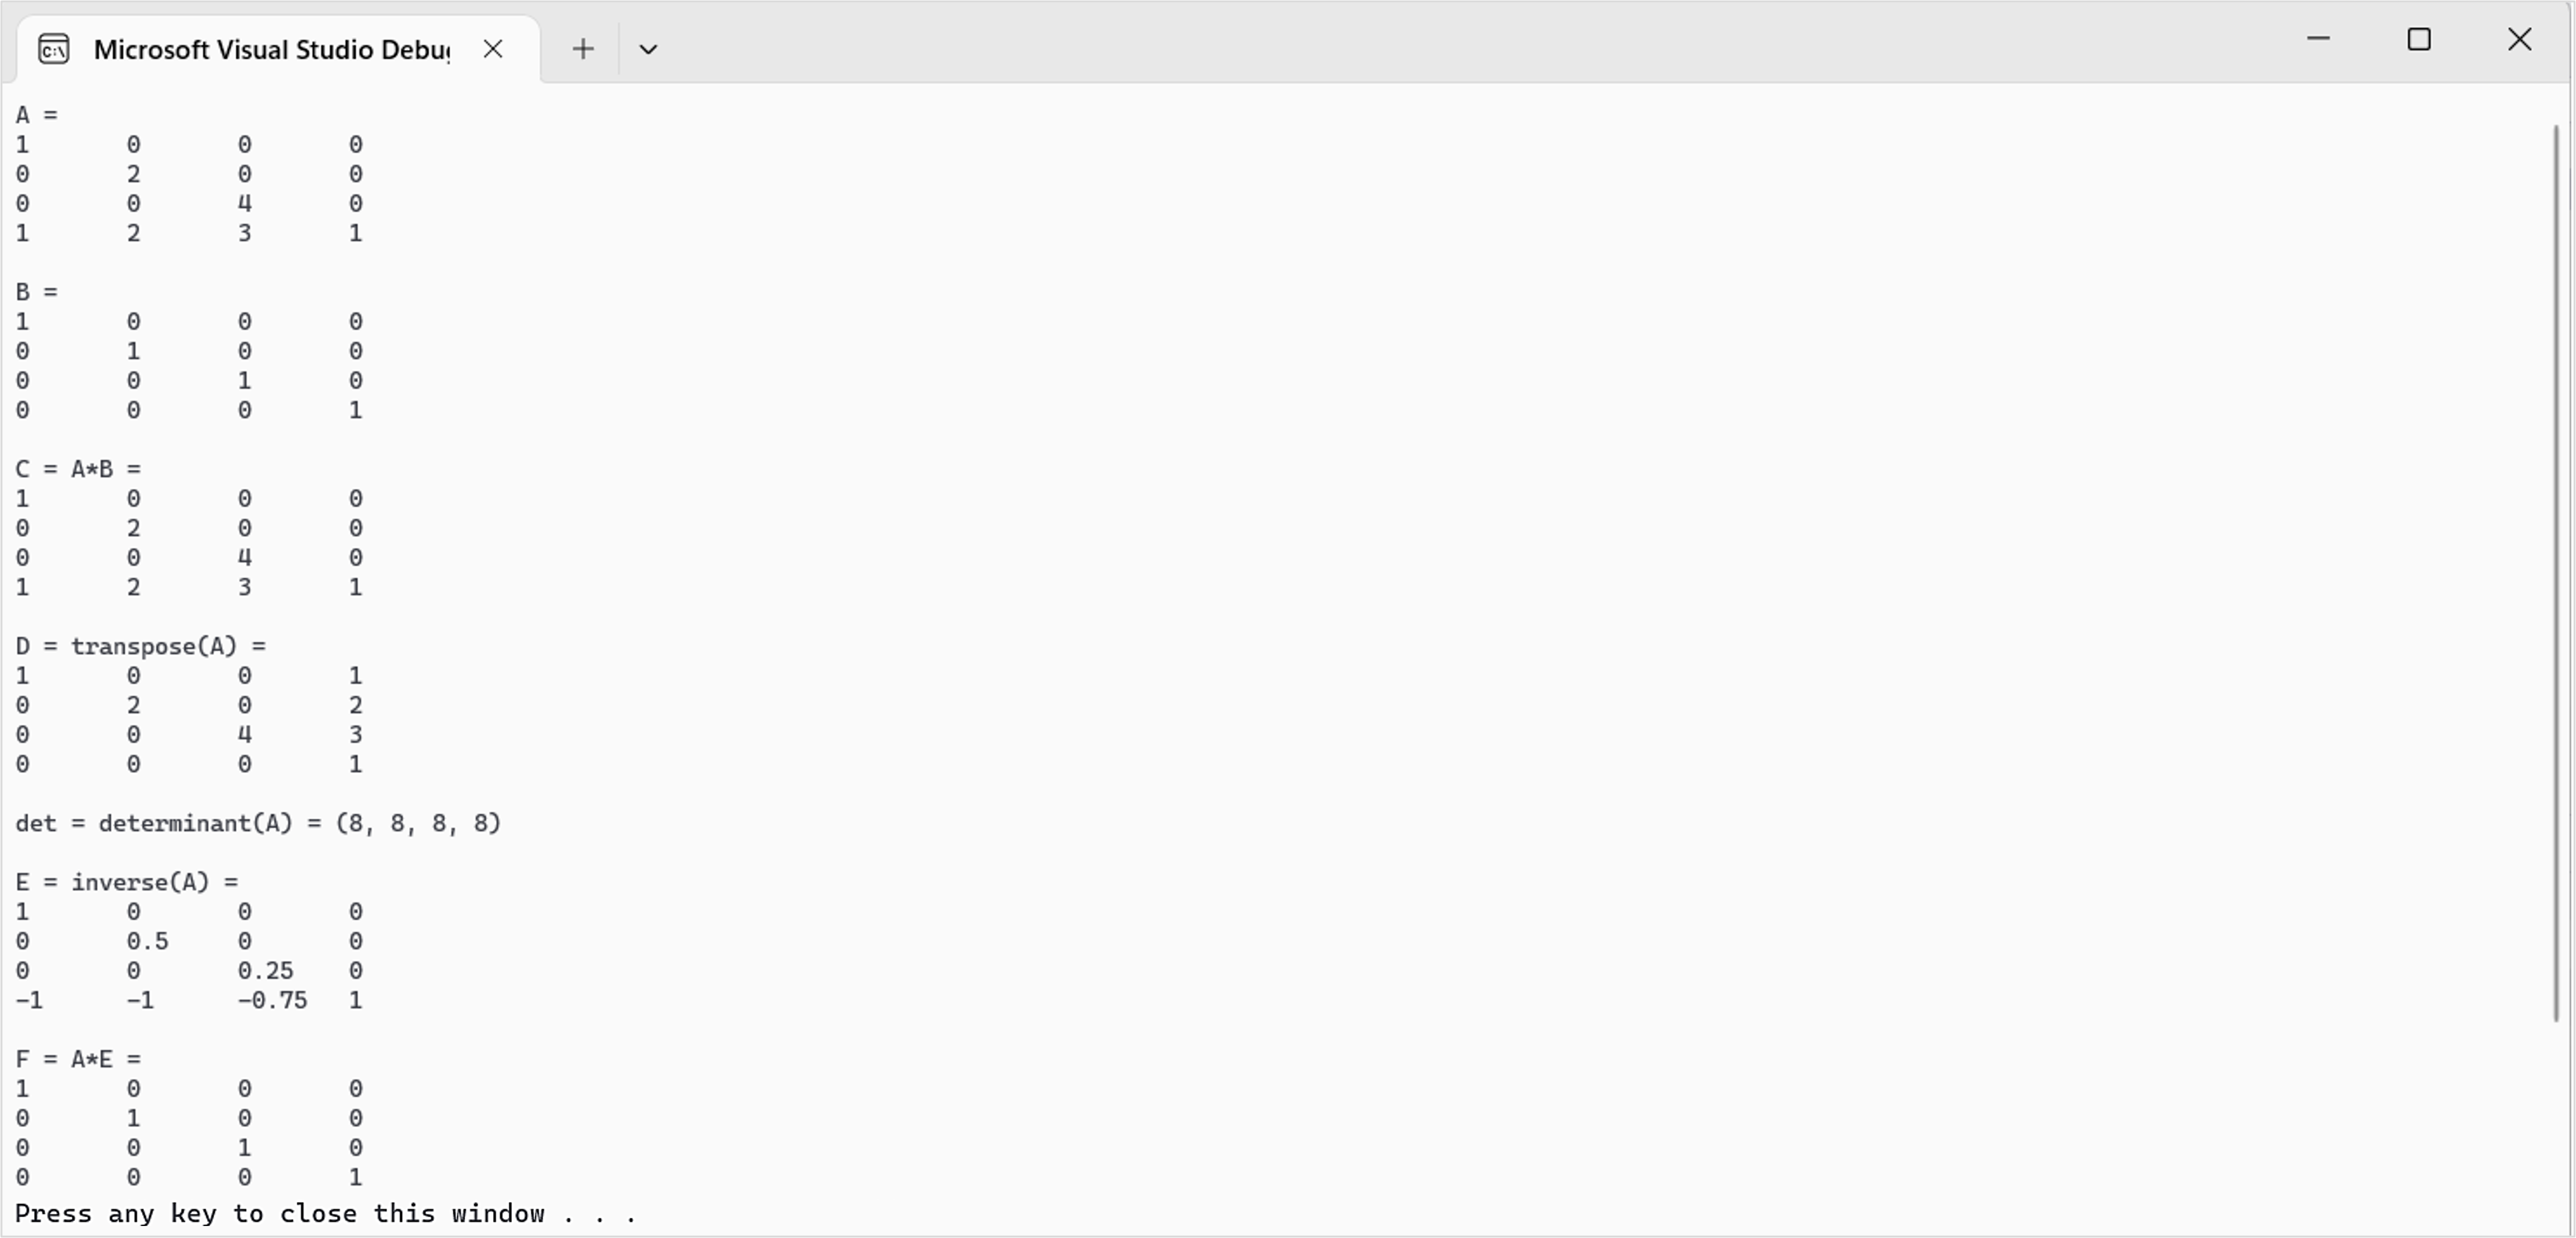
\includegraphics[width=\textwidth]{Images/4/2/4.Session.1.2.1}
            \caption {خروجی برنامه‌ی بالا.}
            \label{fig:4.Session.1.2.1}
        \end{figure}
    \end{spacing}
}
%-----------------------------------------------------------------------------------------------------------%
\newpage


\section{\textbf{خلاصه}}
\label{sec:2.9}
{
    \Large
    \begin{spacing}{1.5}
        \begin{enumerate}[label=\textbf{\arabic*}.]
            \item {$\textbf{A}$ ماتریس $m\times n$، یک آرایه مستطیلی از اعداد حقیقی با $m$ ردیف و $n$ ستون است.
            دو ماتریس با ابعاد یکسان اگر و تنها اگر اجزای متناظر آن‌ها برابر باشند، مساوی هستند.
            ما دو ماتریس با ابعاد یکسان را با اضافه کردن عناصر متناظر آن‌ها جمع می‌کنیم.
            ما یک اسکالر و یک ماتریس را با ضرب اسکالر در هر عنصر در ماتریس ضرب می‌کنیم.}

            \item {اگر $\textbf{A}$ یک ماتریس $m\times n$ و $\textbf{B}$ یک ماتریس $n\times p$ باشد،
            حاصلضرب $\textbf{AB}$ که یک ماتریس $m\times p$ است، با $\textbf{C}$ تعریف می‌شود،
            که در آن ورودی $ij$ ام از $\textbf{C}$ حاصل، با گرفتن ضرب داخلی بردار ردیف $i$ ام $\textbf{A}$ با بردار ستون $j$ ام $\textbf{B}$ به دست می‌آید، یعنی $\textbf{C}^{ij}=\textbf{A}^{i,*}\cdot\textbf{B}^{*,j}$.}

            \item {ضرب ماتریس جابجایی پذیر نیست (به عنوان مثال، به طور کلی $\textbf{AB}\neq\textbf{BA}$). ضرب ماتریس شرکت پذیر است: $(\textbf{AB})\textbf{C}=(\textbf{A})\textbf{BC}$.}

            \item {ترانهاده یک ماتریس با تعویض ردیف‌ها و ستون‌های ماتریس به دست می‌آید.
            بنابراین ترانهاده یک ماتریس $m\times n$ یک ماتریس $n\times m$ است.
            ترانهاده یک ماتریس $\textbf{M}$ را $\textbf{M}^{T}$ نشان می‌دهیم.}

            \item {ماتریس همانی یک ماتریس مربعی است که همه عناصر به جز در امتداد قطر اصلی صفر بوده و عناصر در امتداد قطر اصلی همه یک هستند.}

            \item {دترمینان، \lr{det $\textbf{A}$}، یک تابع ویژه است که یک ماتریس مربعی را دریافت و یک عدد حقیقی را خروجی می‌دهد.
            یک ماتریس مربعی $\textbf{A}$ معکوس پذیر است اگر و تنها اگر $det\textbf{A}\neq 0$ باشد.
            دترمینان در فرمول برای محاسبه معکوس یک ماتریس استفاده می‌شود.}

            \item {از ضرب یک ماتریس در معکوس آن، ماتریس همانی حاصل می‌شود: $\textbf{M}\textbf{M}^{-1}=\textbf{M}^{-1}\textbf{M}=\textbf{I}$.
            معکوس یک ماتریس، اگر وجود داشته باشد، منحصر به فرد است.
            فقط ماتریس‌های مربعی دارای معکوس هستند و حتی در این صورت، ماتریس مربع ممکن است معکوس پذیر نباشد.
            معکوس یک ماتریس را می‌توان با فرمول محاسبه کرد: $\textbf{A}^{-1}=\textbf{A}^{*}/det\textbf{A}$، که در آن $\textbf{A}^{*}$ الحاق است (ترانهاده ماتریس کوفاکتور $\textbf{A}$).}

            \item {ما از نوع ریاضی \texttt{XMMATRIX} در \lr{DirectX} برای توصیف ماتریس $4\times 4$ به طور موثر در کد با استفاده از عملیات \lr{SIMD} استفاده می‌کنیم.
            برای اعضای داده کلاس، ما از کلاس \texttt{XMFLOAT4X4} استفاده می‌کنیم و
            سپس از روش‌های بارگذاری (\texttt{XMLoadFloat4x4}) و ذخیره سازی (\texttt{XMStoreFloat4x4}) برای تبدیل بین \texttt{XMMATRIX} و \texttt{XMFLOAT4X4} به عقب و جلو استفاده می‌کنیم.
            کلاس \texttt{XMMATRIX} عملگرهای حسابی را برای انجام جمع، تفریق، ضرب ماتریس و ضرب اسکالر بارگذاری می‌کند.
            علاوه بر این، کتابخانه ریاضی \lr{DirectX} توابع ماتریس مفید زیر را برای محاسبه ماتریس همانی، ضرب، ترانهاده، دترمینان و معکوس ارائه می‌کند:
            \textbf{\vspace{6pt}}
            \lr{\lstinputlisting[language=C++, firstline=198, lastline=203]{Codes/4.1.2.program.c}}
            }
        \end{enumerate}
    \end{spacing}
}
%-----------------------------------------------------------------------------------------------------------%
\newpage


\section{\textbf{تمارین}}
\label{sec:2.10}
{
    \Large
    \begin{spacing}{1.5}
        \begin{enumerate}[label=\textbf{\arabic*}.]
            \item {معادله ماتریسی روبرو را برای $\textbf{X}$ حل کنید: $\left( \begin{bmatrix}
                                                                                  -2 & 0 \\
                                                                                  1  & 3
            \end{bmatrix}-2\textbf{X}=2\begin{bmatrix}
                                           -2 & 0 \\
                                           1  & 3
            \end{bmatrix} \right)$.}

            \item {ضرب‌های ماتریس زیر را محاسبه کنید:
            \lr{
                \begin{flushleft}
                (a)
                    $\begin{bmatrix}
                         -2 & 0 & 3  \\
                         4  & 1 & -1
                    \end{bmatrix}\begin{bmatrix}
                                     -2 & 1  \\
                                     0  & 6  \\
                                     2  & -3
                    \end{bmatrix}$ \\
                    (b) $\begin{bmatrix}
                             1 & 2 \\
                             3 & 4
                    \end{bmatrix}\begin{bmatrix}
                                     -2 & 0 \\
                                     1  & 1
                    \end{bmatrix}$ \\
                    (c) $\begin{bmatrix}
                             2 & 0  & 2  \\
                             0 & -1 & -3 \\
                             0 & 0  & 1
                    \end{bmatrix}\begin{bmatrix}
                                     1 \\
                                     2 \\
                                     1
                    \end{bmatrix}$
                \end{flushleft}
            }
            }

            \item {معکوس ماتریس‌های زیر را محاسبه کنید:
            \lr{
                \begin{flushleft}
                (a)
                    $[1, 2, 3]$ \\
                    (b) $\begin{bmatrix}
                             x & y \\
                             z & w
                    \end{bmatrix}$ \\
                    (c) $\begin{bmatrix}
                             1 & 2 \\
                             3 & 4 \\
                             5 & 6 \\
                             7 & 8
                    \end{bmatrix}$
                \end{flushleft}
            }
            }

            \item {ترکیب‌های خطی زیر را به‌عنوان ضرب بردار-ماتریس بنویسید:
            \lr{
                \begin{flushleft}
                (a)
                    $\textbf{v}=2(1,2,3)-4(-5,0,-1)+3(2,-2,3)$ \\
                    (b) $\textbf{v}=2(2,-4)+2(1,4)-1(-2,-3)+5(1,1)$
                \end{flushleft}
            } \textbf{\vspace{-6pt}}
            }

            \item {نشان دهید:
                \begin{center}
                    $\textbf{AB}=\begin{bmatrix}
                                     A_{11} & A_{12} & A_{13} \\
                                     A_{21} & A_{22} & A_{23} \\
                                     A_{31} & A_{32} & A_{33}
                    \end{bmatrix}\begin{bmatrix}
                                     B_{11} & B_{12} & B_{13} \\
                                     B_{21} & B_{22} & B_{23} \\
                                     B_{31} & B_{32} & B_{33}
                    \end{bmatrix}=\begin{bmatrix}
                                      \leftarrow & \textbf{A}_{1,*}\textbf{B} & \rightarrow \\
                                      \leftarrow & \textbf{A}_{2,*}\textbf{B} & \rightarrow \\
                                      \leftarrow & \textbf{A}_{3,*}\textbf{B} & \rightarrow
                    \end{bmatrix}$
                \end{center}
            }  \\\textbf{\vspace{6pt}}

            \item {نشان دهید:
                \begin{center}
                    $\textbf{Au}=\begin{bmatrix}
                                     A_{11} & A_{12} & A_{13} \\
                                     A_{21} & A_{22} & A_{23} \\
                                     A_{31} & A_{32} & A_{33}
                    \end{bmatrix}\begin{bmatrix}
                                     x \\
                                     y \\
                                     z
                    \end{bmatrix}=x\textbf{A}_{*,1}+y\textbf{A}_{*,2}+z\textbf{A}_{*,3}$
                \end{center}
            }  \\\textbf{\vspace{6pt}}

            \item {ثابت کنید که ضرب خارجی را می‌توان با ضرب ماتریس بیان کرد:
                \begin{center}
                    $\textbf{u}\times\textbf{v}=\begin{bmatrix}
                                                    v_{x} & v_{y} & v_{z}
                    \end{bmatrix}\begin{bmatrix}
                                     0      & u_{z}  & -u_{y} \\
                                     -u_{z} & 0      & u_{x}  \\
                                     u_{y}  & -u_{x} & 0
                    \end{bmatrix}$
                \end{center}
            } \\\textbf{\vspace{6pt}}

            \item {فرض کنید $\textbf{A}=\begin{bmatrix}
                                            2 & 0  & 1  \\
                                            0 & -1 & -3 \\
                                            0 & 0  & 1
            \end{bmatrix}$. آیا $\textbf{B}=\begin{bmatrix}
                                                1/2 & 0  & -1/2 \\
                                                0   & -1 & -3   \\
                                                0   & 0  & 1
            \end{bmatrix}$ معکوس $\textbf{A}$ است؟
            } \\\textbf{\vspace{6pt}}

            \item {فرض کنید $\textbf{A}=\begin{bmatrix}
                                            1 & 2 \\
                                            3 & 4
            \end{bmatrix}$. آیا $\textbf{B}=\begin{bmatrix}
                                                -2  & 1   \\
                                                3/2 & 1/2
            \end{bmatrix}$ معکوس $\textbf{A}$ است؟
            }

            \item {دترمینان‌های ماتریس‌های زیر را بیابید:
                \begin{center}
                    $\begin{bmatrix}
                         21 & -4 \\
                         10 & 7
                    \end{bmatrix}$,
                    $\begin{bmatrix}
                         2 & 0 & 0 \\
                         0 & 3 & 0 \\
                         0 & 0 & 7
                    \end{bmatrix}$
                \end{center}
            } \\\textbf{\vspace{6pt}}

            \item {معکوس ماتریس‌های زیر را بیابید:
                \begin{center}
                    $\begin{bmatrix}
                         21 & -4 \\
                         10 & 7
                    \end{bmatrix}$,
                    $\begin{bmatrix}
                         2 & 0 & 0 \\
                         0 & 3 & 0 \\
                         0 & 0 & 7
                    \end{bmatrix}$
                \end{center}
            } \\\textbf{\vspace{6pt}}

            \item {آیا ماتریس زیر معکوس پذیر است؟
                \begin{center}
                    $\begin{bmatrix}
                         1 & 2 & 3 \\
                         0 & 4 & 5 \\
                         0 & 0 & 0
                    \end{bmatrix}$
                \end{center}
            } \\\textbf{\vspace{6pt}}

            \item {نشان دهید که $(\textbf{A}^{-1})^{T}=(\textbf{A}^{T})^{-1}$، با فرض اینکه $\textbf{A}$ معکوس پذیر است.}  \\\textbf{\vspace{6pt}}

            \item {فرض کنید $\textbf{A}$ و $\textbf{B}$ ماتریس $n\times n$ باشند.
            یک واقعیت ثابت شده در کتاب‌های جبر خطی این است که $det\textbf{AB}=det\textbf{A}\cdot det\textbf{B}$.
            از این واقعیت به همراه $det\textbf{I}=1$ برای اثبات $\textbf{A}^{-1}=\frac{\displaystyle 1}{\displaystyle det\textbf{A}}$ استفاده کنید،
            با فرض اینکه $\textbf{A}$ معکوس پذیر است.} \\\textbf{\vspace{6pt}}

            \item {ثابت کنید که دترمینان دوبعدی  $\begin{bmatrix}
                                                      u_{x} & u_{y} \\
                                                      v_{x} & v_{y}
            \end{bmatrix}$ مساحت علامت متوازی الاضلاع را می‌دهد که با $\textbf{u}=(u_{x},u_{y})$ و $\textbf{v}=(v_{x},v_{y})$ پوشیده شده است.
            نتیجه مثبت است اگر $\textbf{u}$ را بتوان در خلاف جهت عقربه‌های ساعت بچرخانیم تا با $\textbf{v}$ با زاویه $\theta\in(0,\pi)$ منطبق شود، و در غیر‌این صورت منفی است.
                \begin{figure}[H]
                    \centering
                    \setlength{\belowcaptionskip}{-10pt}
                    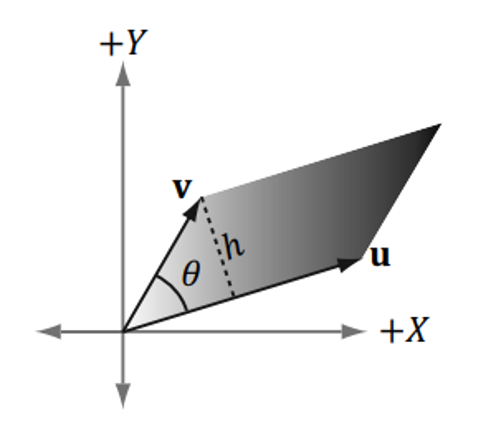
\includegraphics[width=0.4\textwidth]{Images/4/2/4.Session.1.2.2}
                    \label{fig:4.Session.1.2.2}
                \end{figure}
            }

            \item {مساحت متوازی الاضلاع را بیابید که با موارد زیر پوشیده شده باشد:
            \lr{\begin{flushleft}
            (a)
                    $\textbf{u}=(3,0), \textbf{v}=(1,1)$\\
                    (b) $\textbf{u}=(-1,-1), \textbf{v}=(0,1)$
            \end{flushleft}}
            }

            \item {فرض کنید $\textbf{A}=\begin{bmatrix}
                                            A_{11} & A_{12} \\
                                            A_{21} & A_{22}
            \end{bmatrix}$، $\textbf{B}=\begin{bmatrix}
                                            B_{11} & B_{12} \\
                                            B_{21} & B_{22}
            \end{bmatrix}$ و $\textbf{C}=\begin{bmatrix}
                                             C_{11} & C_{12} \\
                                             C_{21} & C_{22}
            \end{bmatrix}$ نشان دهید که $\textbf{A}(\textbf{BC})=(\textbf{AB})\textbf{C}$.
            این نشان می‌دهد که ضرب ماتریس برای ماتریس‌های $2\times 2$ شرکت پذیر است.
                (در واقع، هر زمان که ضرب تعریف شود، ضرب ماتریس برای ماتریس‌های با اندازه عمومی شرکت پذیر است.)} \\\textbf{\vspace{6pt}}

            \item {یک برنامه کامپیوتری بنویسید که ترانهاده یک ماتریس $m\times n$ را بدون استفاده از \lr{DirectX Math} محاسبه کند
                (فقط از آرایه‌ای از آرایه‌ها در \lr{C++} استفاده کنید).} \\\textbf{\vspace{6pt}}

            \item {یک برنامه کامپیوتری بنویسید که دترمینان و معکوس ماتریس‌های $4\times 4$ را بدون استفاده از \lr{DirectX Math} محاسبه کند
                (فقط از آرایه‌ای از آرایه‌ها در \lr{C++} استفاده کنید).}
        \end{enumerate}
    \end{spacing}
}